%!TEX root = ../dokumentation.tex
\section{Projekorganisation}

\begin{figure}[!ht]
\begin{center}
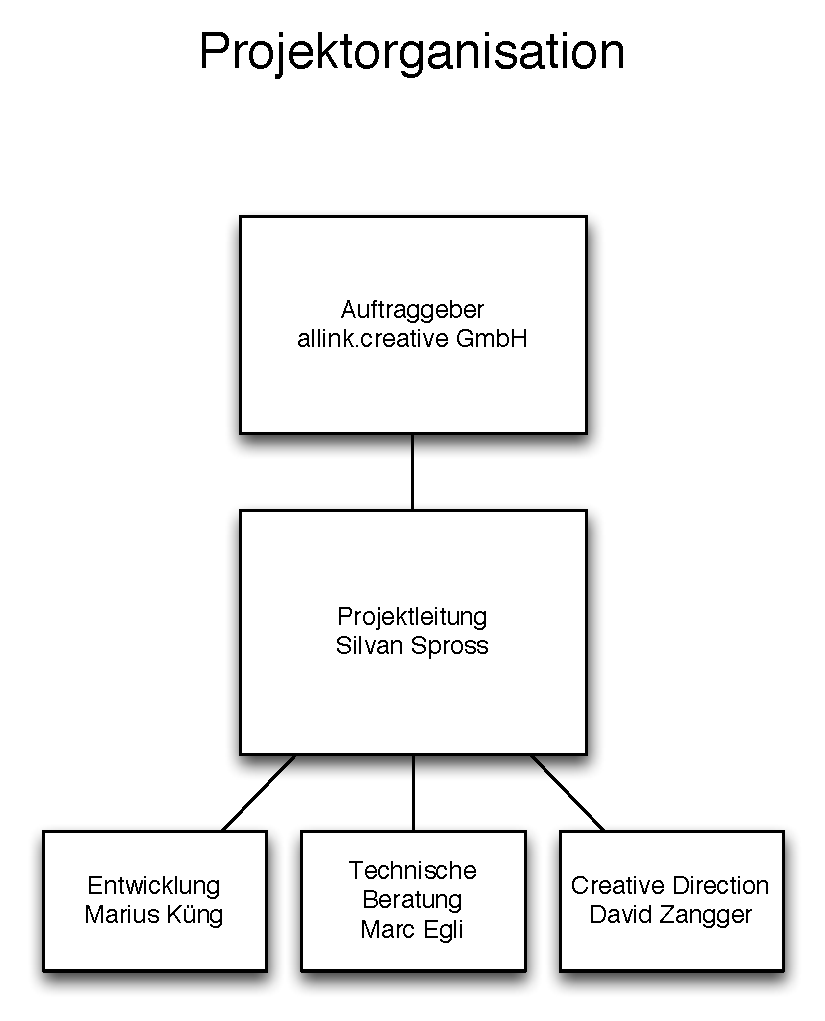
\includegraphics[width=0.5\textwidth,angle=0]{./bilder/01_projektorganisation.pdf}
\caption[Projekorganisation]{Projekorganisation\footnotemark}
\end{center}
\end{figure}
\footnotetext{Eigene Darstellung}

\section{Vorkenntnisse}

Technologien
\begin{itemize}
    \item Python Grundkenntnisse
    \item Django fortgeschrittene Kenntnisse
    \item Piston Grundkenntnisse
    \item jQuery fortgeschrittene Kenntnisse
    \item HTML5 gute Kenntnisse
    \item CSS3 gute Kenntnisse
    \item AJAX fortgeschrittene Kenntnisse\\
\end{itemize}

Anwendungen
\begin{itemize}
    \item Mehrere komplette Webauftritte realisiert
    \item Applikationen in Django erstellt (News, Blog, Produkteübersicht)
    \item Schnittstellen programmiert (XML, JSON)
    \item Per AJAX dynamische Inhalte laden und einfügen
    \item Dynamische Formulare abschicken und Request entgegenehmen
    \item DOM-Elemente manipulieren, per Events steuern
\end{itemize}
    
\section{Vorarbeiten}
Ich habe, um einen ersten Eindruck über die Funktionalität zu erhalten, den bestehenden yatplaner ausprobiert.
Ansonsten fand keine explizite Vorarbeit statt.

\section{Firmenstandards}
\begin{itemize}
    \item Betriebsystem: Mac OS X
    \item Editor: Textmate
    \item Entwicklungsumgebung: Python, Django (Python-Framework für Webapplikationen)
    \item Lokale Testumgebung: Django Server
    \item Deployment: per fabric-script auf Apache-Server
    \item Versionierung: Git, auf Github veröffentlicht
\end{itemize}
Die folgende Grafik beschreibt einen Standardaufbau wie ein Git-Repository gegliedert ist.
    \begin{figure}[!ht]
    \begin{center}
    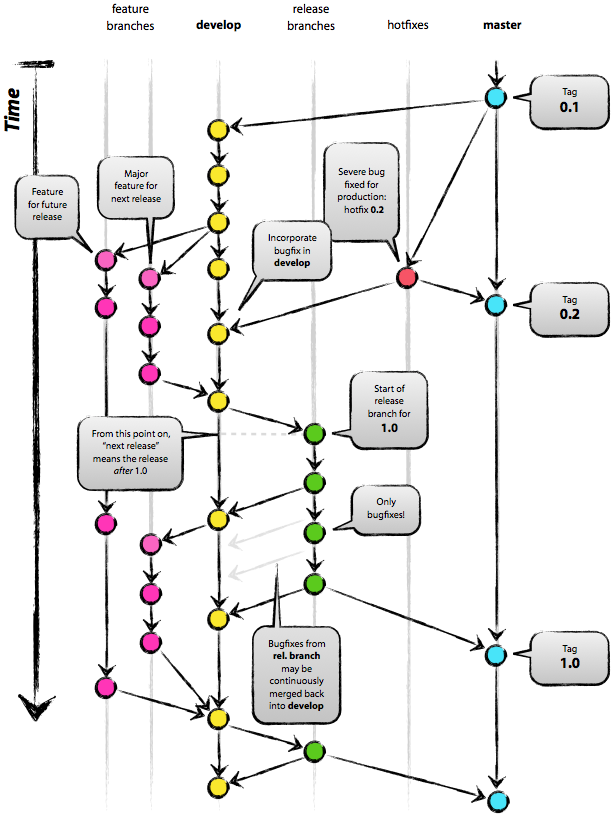
\includegraphics[width=0.99\textwidth,angle=0]{./bilder/git.png}
    \caption{A successful Git branching model von Vincent Driessen}
    \end{center}
    \end{figure}

